\chapter{Background}
\label{chp:Background}
This chapter first presents the background knowledge required to understand the thesis. The first sections describes the characteristics of lights in general. The second section explains how a model can be made which describes the reflection of light. The third section explains how a light can be dimmed, and how this affects the total amount of light outputted, the amount of light sensed by electronics and the human experience.

\section{Characteristics of a lights}
\label{sec:Characteristics of light}
Before reading this thesis, a basic understanding of photometry is required. For this reason, this section will first introduce the the units and measures used in this document, followed by the most used method for modelling and calculating these measures.

\subsection{Units and measures of light}

\begin{table}[h]
	\centering
	\label{Photometric_measures}
	\begin{tabular}{llll}
		Name                                   & Symbol  & unit                          & Description                                        \\ \hline
		\multicolumn{1}{l|}{Radiant flux}     & $\Phi_e$ & $W$                         & Radiant energy per unit time                        \\
		\multicolumn{1}{l|}{Luminous flux}     & $\Phi_v$ & $lm$                         & Luminous energy per unit time                       \\
		\multicolumn{1}{l|}{Luminous intensity}& $I_v$    & $lm/sr (= cd)$                         & Wavelength-weighted power emitted by a light source in a particular detection per solid angle\\
		\multicolumn{1}{l|}{Illuminance}       & $E_v$    & $lm/m^2 (= lx)$              & Amount of luminous flux impinging a surface       \\
		\multicolumn{1}{l|}{Luminous energy}   & $Q_v$    & $lm*s$                       & Total amount of luminous flux outputted over time \\
		\multicolumn{1}{l|}{Luminous exposure} & $H_v$    & $lx*s$                       & Total amount of  illuminance impinging on a surface over time  \\
	\end{tabular}
	\caption{summary of measures, units and symbols used in this thesis}
\end{table}

\begin{table}[h]
	\centering
	\label{Model_symbols}
	\begin{tabular}{llll}
		Name                                   & Symbol  & unit                          & Description                                        \\ \hline
		\multicolumn{1}{l|}{Light uniformity}  & $U_0$    & -                            & $E_{min}/E_{mean}$  \\
		\multicolumn{1}{l|}{Reflection coefficient}& $\rho$ & -                          & wavelength dependent surface reflection ratio\\
		\multicolumn{1}{l|}{Albedo}            & $\alpha$ & -                            & Impinging intensity / reflected intensity\\
		\multicolumn{1}{l|}{Exit angle}        & $\phi$   & rad                          & Exit angle with respect to the normal of the reflective surface\\
		\multicolumn{1}{l|}{Incidence angle}   & $\theta$ & rad                          & Incidence angle with respect to the normal of the reflective surface\\
	\end{tabular}
	\caption{summary of measures, units and symbols used for modeling light}
\end{table}

\begin{table}[h]
	\centering
	\label{Algorithm_symbols}
	\begin{tabular}{llll}
		Name                                   & Symbol   & unit   & Description                                        \\ \hline
		\multicolumn{1}{l|}{Standard deviation}& $\sigma$ & -      & Measure of variance over a set of values  \\
		\multicolumn{1}{l|}{Mean}              & $\mu$ or $\overline{X}$ & -      & average of a set of values  \\
		\multicolumn{1}{l|}{n}                 & $n$ & -      & Number of samples in the N section of the algorithm \\
		\multicolumn{1}{l|}{d}                 & $d$ & -      & Number of samples in the D section of the algorithm  \\
		\multicolumn{1}{l|}{m}                 & $m$ & -      & Number of samples in the M section of the algorithm \\
		\multicolumn{1}{l|}{Threshold value}   & $T$ & -      & Value determining the detection threshold \\
		\multicolumn{1}{l|}{Scale value}       & $ss$ & -     & Value changing n based on the noise in the current signal \\
	\end{tabular}
	\caption{summary of measures, units and symbols used in the algorithm section}
\end{table}

\subsection{Modelling a light}

\begin{figure}
	\centering     %%% not \center
	\subfigure[Specs of an LED]{\label{fig:Specs_a}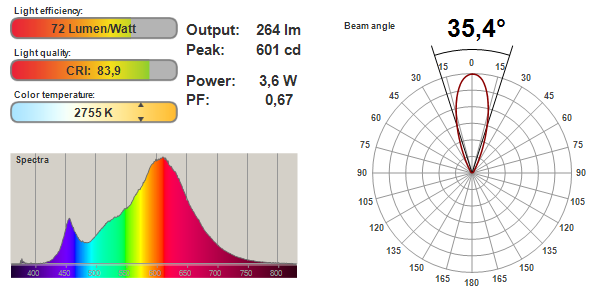
\includegraphics[width=68mm]{pics/LED_specs.png}}
	\subfigure[Caclculated intensity pattern ]{\label{fig:Specs_b}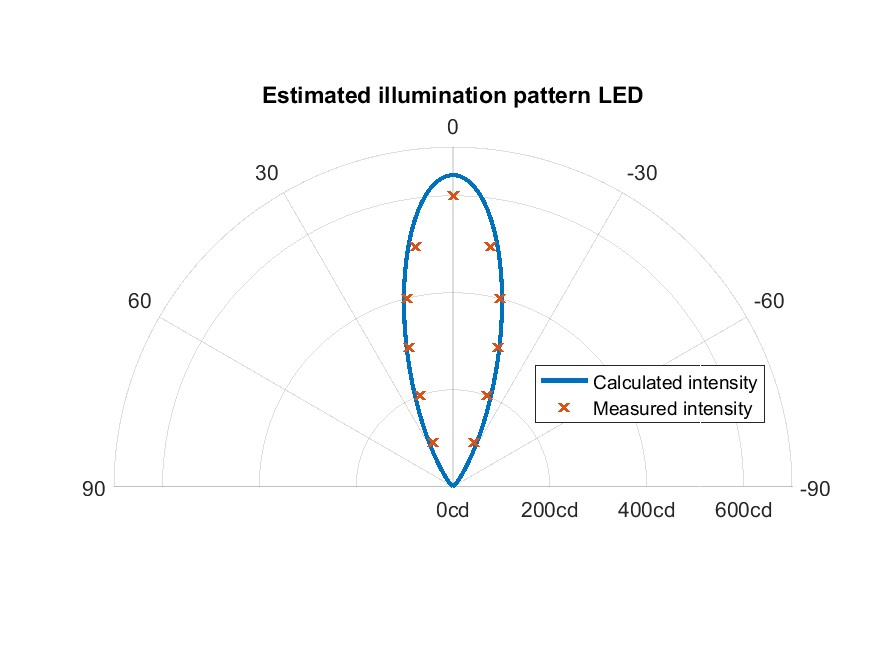
\includegraphics[width=52mm]{pics/polarplot_LED.png}}
	\caption{Figure a shows measured specifications of an LED \cite{lamptest} where Figure b shows the estimated illumination pattern of the same LED.}
\end{figure}

\label{subsec:Modeling_of_light}
Light sources in optics are typically modelled as a point in spaces, emitting light in a Lambertian radiation pattern [x]. This pattern describes how much light leaves a light-source at angle $\phi$ and can be calculated with:
\begin{equation}
\label{eq:I(phi)}
I(\phi)=\Phi_{lum}\frac{m+1}{2\pi}cos^m(\phi)
\end{equation}
where $\Phi_{lum}$ is the luminous flux of the light and $m$ is the order of lambertian emission calculated with $m = -1 / log_2(cos\varphi_{1/2})$ where $\varphi_{1/2}$ is the angle where light is leaving the luminaire at half power. 

With equation \ref{eq:I(phi)} we can now estimate the illumination pattern of any LED when the luminous flux and half power angle are known. This can be done  for example with the LED in figure \ref{fig:Specs_a}. If we choose $\Phi_{lum} = 264 lm$ and $\varphi_{1/2} = 17.7^{\circ}$ then we obtain the pattern shown in figure \ref{fig:Specs_b} which closely matches the measured irradiation pattern.

\begin{equation}
\label{eq:Ehor}
E_{hor}=\frac{I(\phi)\cos(\theta)}{d^2} \to E_{hor}(x,y,z) = \frac{I(\phi(x,y,z))\cos(\theta(x,y,z))}{x^2+y^2+z^2}
\end{equation}

\subsection{Modelling a reflection}
\label{subsec:Modeling_of_reflection}
Now the illumination pattern of a light bulb is known, we are able to calculate how much a light is illuminating a surface with equation \ref{eq:Ehor}. Some of the light will reflect back in the environment while the rest of the light is absorbed by the material and turned another form of energy (typically heat). The total amount of light reflecting back in the environment can be calculated with the surface reflection coefficient $p(\lambda)$. $p$ has a different value for each wavelength $\lambda$ as not every material reflects the same colour of light. An example reflection coefficient can be seen in figure X.

\begin{equation}
\label{eq:R_total}
R_{total} = {E_hor} * p(\lambda)
\end{equation}

The next step is to determine the directions of the reflection. How much light will be reflected in what directions? There are three ways light can be distributed when reflecting of a surface: Specular, spread and diffuse. A visual representation of each of these reflection patterns is shown in Figure \ref{fig:phong}. Each pattern will be discussed briefly.

The \textbf{specular pattern} 

The \textbf{diffuse pattern} is the

The \textbf{spread pattern} is

 is, it can be approximated by setting \textit{m} to infinite from eq x.

Some materials have both emit a lambertian pattern and spread pattern. these can be combined with ratio $r_d$ (amount of diffuse reflection), as seen in equation x. This eqation can now be used to model any reflection $R$, as long as the 

\begin{equation}
\label{eq:Reflection}
I = P_{I}\rho(\lambda)\left[ r_{d} \frac{1}{\pi}\cos(\phi_2)+ (1-r_{d})\frac{m+1}{2\pi}\cos^m(\phi_2'-\phi_2) \right]
\end{equation}

\begin{figure}
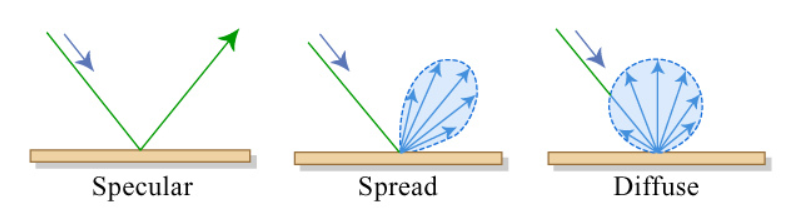
\includegraphics[width=\textwidth]{pics/3_reflections.png}
\caption{The possible ways for light to reflect when it hits a surface \cite{3reflections}}
\label{fig:phong}
%source https://www.researchgate.net/figure/221895787_fig3_Fig-3-Phong-reflection-model-a-diffuse-reflection-light-b-specular-reflection
\end{figure}

\begin{equation}
\label{eq:PD}
P_{PD}=\frac{P_{I}\cos(\theta)}{d^2} rec \left( \frac{\theta}{FOV} \right)
\end{equation}

\begin{equation}
\label{eq:total}
E_{PD}= E_{hor} * p(\lambda) * R(r_d,\phi_2,\phi_2') * \frac{cos(\theta_2)}{d_2^2}
\end{equation}

\section{Dimming and its consequences}
\label{sec:Dimming and its consequences}

Explain what dimming of light is and means\\

\subsection{Types of dimming}
Explain analog dimming (intensity)\\
\\
Explain digital dimming (pwm)\\

\subsection{Limits of dimming}
Explain the limits analog dimming:\\
   - At some point there is not enough current to turn on the lights.\\
   - Reduces range\\
Explain the limits of pwm dimming\\
   - There is a time required for the LED to turn on\\
   - There is a time required for the let to turn off\\
   - Making the total on time \textbf{a bit} too short results in a huge variance in light emitted\\
   - Making the total on time \textbf{a lot} too short results in no light\\
   \\
   Note that this does not reduce range
   
LedResponse.png
\begin{figure}[!h]
	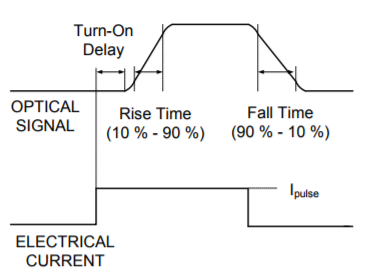
\includegraphics[width=\textwidth]{pics/LedResponse.png}
	\caption{Realistic light response.}
	\label{fig:LedOnTime}
	%source https://www.osram-os.com/Graphics/XPic5/00135349_0.pdf/High-Speed%20Switching%20of%20IR-LEDs.pdf
\end{figure}

